% Options for packages loaded elsewhere
\PassOptionsToPackage{unicode}{hyperref}
\PassOptionsToPackage{hyphens}{url}
%
\documentclass[
]{article}
\usepackage{amsmath,amssymb}
\usepackage{lmodern}
\usepackage{ifxetex,ifluatex}
\ifnum 0\ifxetex 1\fi\ifluatex 1\fi=0 % if pdftex
  \usepackage[T1]{fontenc}
  \usepackage[utf8]{inputenc}
  \usepackage{textcomp} % provide euro and other symbols
\else % if luatex or xetex
  \usepackage{unicode-math}
  \defaultfontfeatures{Scale=MatchLowercase}
  \defaultfontfeatures[\rmfamily]{Ligatures=TeX,Scale=1}
\fi
% Use upquote if available, for straight quotes in verbatim environments
\IfFileExists{upquote.sty}{\usepackage{upquote}}{}
\IfFileExists{microtype.sty}{% use microtype if available
  \usepackage[]{microtype}
  \UseMicrotypeSet[protrusion]{basicmath} % disable protrusion for tt fonts
}{}
\makeatletter
\@ifundefined{KOMAClassName}{% if non-KOMA class
  \IfFileExists{parskip.sty}{%
    \usepackage{parskip}
  }{% else
    \setlength{\parindent}{0pt}
    \setlength{\parskip}{6pt plus 2pt minus 1pt}}
}{% if KOMA class
  \KOMAoptions{parskip=half}}
\makeatother
\usepackage{xcolor}
\IfFileExists{xurl.sty}{\usepackage{xurl}}{} % add URL line breaks if available
\IfFileExists{bookmark.sty}{\usepackage{bookmark}}{\usepackage{hyperref}}
\hypersetup{
  pdftitle={Ejercicios Tema 1. Segunda Entrega.},
  hidelinks,
  pdfcreator={LaTeX via pandoc}}
\urlstyle{same} % disable monospaced font for URLs
\usepackage[margin=1in]{geometry}
\usepackage{color}
\usepackage{fancyvrb}
\newcommand{\VerbBar}{|}
\newcommand{\VERB}{\Verb[commandchars=\\\{\}]}
\DefineVerbatimEnvironment{Highlighting}{Verbatim}{commandchars=\\\{\}}
% Add ',fontsize=\small' for more characters per line
\usepackage{framed}
\definecolor{shadecolor}{RGB}{248,248,248}
\newenvironment{Shaded}{\begin{snugshade}}{\end{snugshade}}
\newcommand{\AlertTok}[1]{\textcolor[rgb]{0.94,0.16,0.16}{#1}}
\newcommand{\AnnotationTok}[1]{\textcolor[rgb]{0.56,0.35,0.01}{\textbf{\textit{#1}}}}
\newcommand{\AttributeTok}[1]{\textcolor[rgb]{0.77,0.63,0.00}{#1}}
\newcommand{\BaseNTok}[1]{\textcolor[rgb]{0.00,0.00,0.81}{#1}}
\newcommand{\BuiltInTok}[1]{#1}
\newcommand{\CharTok}[1]{\textcolor[rgb]{0.31,0.60,0.02}{#1}}
\newcommand{\CommentTok}[1]{\textcolor[rgb]{0.56,0.35,0.01}{\textit{#1}}}
\newcommand{\CommentVarTok}[1]{\textcolor[rgb]{0.56,0.35,0.01}{\textbf{\textit{#1}}}}
\newcommand{\ConstantTok}[1]{\textcolor[rgb]{0.00,0.00,0.00}{#1}}
\newcommand{\ControlFlowTok}[1]{\textcolor[rgb]{0.13,0.29,0.53}{\textbf{#1}}}
\newcommand{\DataTypeTok}[1]{\textcolor[rgb]{0.13,0.29,0.53}{#1}}
\newcommand{\DecValTok}[1]{\textcolor[rgb]{0.00,0.00,0.81}{#1}}
\newcommand{\DocumentationTok}[1]{\textcolor[rgb]{0.56,0.35,0.01}{\textbf{\textit{#1}}}}
\newcommand{\ErrorTok}[1]{\textcolor[rgb]{0.64,0.00,0.00}{\textbf{#1}}}
\newcommand{\ExtensionTok}[1]{#1}
\newcommand{\FloatTok}[1]{\textcolor[rgb]{0.00,0.00,0.81}{#1}}
\newcommand{\FunctionTok}[1]{\textcolor[rgb]{0.00,0.00,0.00}{#1}}
\newcommand{\ImportTok}[1]{#1}
\newcommand{\InformationTok}[1]{\textcolor[rgb]{0.56,0.35,0.01}{\textbf{\textit{#1}}}}
\newcommand{\KeywordTok}[1]{\textcolor[rgb]{0.13,0.29,0.53}{\textbf{#1}}}
\newcommand{\NormalTok}[1]{#1}
\newcommand{\OperatorTok}[1]{\textcolor[rgb]{0.81,0.36,0.00}{\textbf{#1}}}
\newcommand{\OtherTok}[1]{\textcolor[rgb]{0.56,0.35,0.01}{#1}}
\newcommand{\PreprocessorTok}[1]{\textcolor[rgb]{0.56,0.35,0.01}{\textit{#1}}}
\newcommand{\RegionMarkerTok}[1]{#1}
\newcommand{\SpecialCharTok}[1]{\textcolor[rgb]{0.00,0.00,0.00}{#1}}
\newcommand{\SpecialStringTok}[1]{\textcolor[rgb]{0.31,0.60,0.02}{#1}}
\newcommand{\StringTok}[1]{\textcolor[rgb]{0.31,0.60,0.02}{#1}}
\newcommand{\VariableTok}[1]{\textcolor[rgb]{0.00,0.00,0.00}{#1}}
\newcommand{\VerbatimStringTok}[1]{\textcolor[rgb]{0.31,0.60,0.02}{#1}}
\newcommand{\WarningTok}[1]{\textcolor[rgb]{0.56,0.35,0.01}{\textbf{\textit{#1}}}}
\usepackage{graphicx}
\makeatletter
\def\maxwidth{\ifdim\Gin@nat@width>\linewidth\linewidth\else\Gin@nat@width\fi}
\def\maxheight{\ifdim\Gin@nat@height>\textheight\textheight\else\Gin@nat@height\fi}
\makeatother
% Scale images if necessary, so that they will not overflow the page
% margins by default, and it is still possible to overwrite the defaults
% using explicit options in \includegraphics[width, height, ...]{}
\setkeys{Gin}{width=\maxwidth,height=\maxheight,keepaspectratio}
% Set default figure placement to htbp
\makeatletter
\def\fps@figure{htbp}
\makeatother
\setlength{\emergencystretch}{3em} % prevent overfull lines
\providecommand{\tightlist}{%
  \setlength{\itemsep}{0pt}\setlength{\parskip}{0pt}}
\setcounter{secnumdepth}{-\maxdimen} % remove section numbering
\ifluatex
  \usepackage{selnolig}  % disable illegal ligatures
\fi

\title{Ejercicios Tema 1. Segunda Entrega.}
\author{}
\date{\vspace{-2.5em}}

\begin{document}
\maketitle

\textbf{\emph{Pau Vives, Harold Cruz, Samuel de Paúl}}

\textbf{\emph{PARTE I}}

\emph{1.Calcula la tasa de asesinatos por cada 100000 habitantes para
cada estado y almacénela en un objeto llamado murder\_rate. Luego, usa
operadores lógicos para crear un vector lógico llamado low que nos dice
qué entradas de murder\_rate son inferiores a 1.}

\begin{Shaded}
\begin{Highlighting}[]
\CommentTok{\#Importamos los datos}
\FunctionTok{data}\NormalTok{(murders)}

\CommentTok{\#Calculamos la tasa}
\NormalTok{murder\_rate }\OtherTok{\textless{}{-}}\NormalTok{ murders}\SpecialCharTok{$}\NormalTok{total }\SpecialCharTok{/}\NormalTok{ murders}\SpecialCharTok{$}\NormalTok{population }\SpecialCharTok{*} \DecValTok{100000}

\CommentTok{\#entradas inferiores a 1:}
\NormalTok{low }\OtherTok{\textless{}{-}}\NormalTok{ murder\_rate }\SpecialCharTok{\textless{}} \DecValTok{1}
\end{Highlighting}
\end{Shaded}

\emph{2.Ahora usa los resultados del ejercicio anterior y la función
which para determinar los índices de murder\_rate asociados con valores
inferiores a 1.}

\begin{Shaded}
\begin{Highlighting}[]
\CommentTok{\#Directamente buscamos en qué posiciones están los TRUE del vector lógico del ejercicio anterior}
\NormalTok{ind }\OtherTok{=} \FunctionTok{which}\NormalTok{(low }\SpecialCharTok{==} \ConstantTok{TRUE}\NormalTok{)}
\NormalTok{ind}
\end{Highlighting}
\end{Shaded}

\begin{verbatim}
##  [1] 12 13 16 20 24 30 35 38 42 45 46 51
\end{verbatim}

\emph{3.Usa los resultados del ejercicio anterior para indicar los
nombres de los estados con tasas de asesinatos inferiores a 1.}

\begin{Shaded}
\begin{Highlighting}[]
\CommentTok{\#Escogemos de la columna de los estados aquellos dados por la lista de índices del ejercicio anterior}
\NormalTok{murders}\SpecialCharTok{$}\NormalTok{state[ind]}
\end{Highlighting}
\end{Shaded}

\begin{verbatim}
##  [1] "Hawaii"        "Idaho"         "Iowa"          "Maine"        
##  [5] "Minnesota"     "New Hampshire" "North Dakota"  "Oregon"       
##  [9] "South Dakota"  "Utah"          "Vermont"       "Wyoming"
\end{verbatim}

\emph{4.Ahora extiende el código de los ejercicios 2 y 3 para indicar
los estados del noreste con tasas de asesinatos inferiores a 1.
Sugerencia: use el vector lógico predefinido low y el operador lógico
\&.}

\begin{Shaded}
\begin{Highlighting}[]
\NormalTok{murders}\SpecialCharTok{$}\NormalTok{state[low }\SpecialCharTok{\&}\NormalTok{ murders}\SpecialCharTok{$}\NormalTok{region }\SpecialCharTok{==} \StringTok{"Northeast"}\NormalTok{]}
\end{Highlighting}
\end{Shaded}

\begin{verbatim}
## [1] "Maine"         "New Hampshire" "Vermont"
\end{verbatim}

\emph{5.En un ejercicio anterior, calculamos la tasa de asesinatos para
cada estado y el promedio de estos números. ¿Cuántos estados están por
debajo del promedio?.}

\begin{Shaded}
\begin{Highlighting}[]
\CommentTok{\#Calculamos la tasa media}
\NormalTok{murder\_mean }\OtherTok{\textless{}{-}} \FunctionTok{mean}\NormalTok{(murder\_rate)}
\NormalTok{murder\_mean}
\end{Highlighting}
\end{Shaded}

\begin{verbatim}
## [1] 2.779125
\end{verbatim}

\begin{Shaded}
\begin{Highlighting}[]
\CommentTok{\#Creamos un vector lógico que nos dice, de las entradas de murder\_rate, cuáles están por debajo de la tasa media, y utilizamos sum para ver de cuantos estados se trata}
\NormalTok{below\_mean }\OtherTok{\textless{}{-}}\NormalTok{ murder\_rate}\SpecialCharTok{\textless{}}\NormalTok{murder\_mean}
\FunctionTok{sum}\NormalTok{(below\_mean)}
\end{Highlighting}
\end{Shaded}

\begin{verbatim}
## [1] 27
\end{verbatim}

\emph{6.Usa la función match para identificar los estados con
abreviaturas AK, MI e IA. Sugerencia: comienza definiendo un índice de
las entradas de murders\$abb que coinciden con las tres abreviaturas.
Entonces usa el operador {[} para extraer los estados.}

\begin{Shaded}
\begin{Highlighting}[]
\NormalTok{ind }\OtherTok{\textless{}{-}} \FunctionTok{match}\NormalTok{(}\FunctionTok{c}\NormalTok{(}\StringTok{"AK"}\NormalTok{, }\StringTok{"MI"}\NormalTok{, }\StringTok{"IA"}\NormalTok{), murders}\SpecialCharTok{$}\NormalTok{abb)}
\NormalTok{murders}\SpecialCharTok{$}\NormalTok{state[ind]}
\end{Highlighting}
\end{Shaded}

\begin{verbatim}
## [1] "Alaska"   "Michigan" "Iowa"
\end{verbatim}

\emph{7.Utiliza el operador \%in\% para crear un vector lógico que
responda a la pregunta: ¿cuáles de las siguientes son abreviaturas
reales: MA, ME, MI, MO, MU?}

\begin{Shaded}
\begin{Highlighting}[]
\CommentTok{\#Creamos el vector lógico como se indica tomamos los índices correspondientes}
\NormalTok{abbs }\OtherTok{\textless{}{-}} \FunctionTok{c}\NormalTok{(}\StringTok{"MA"}\NormalTok{,}\StringTok{"ME"}\NormalTok{,}\StringTok{"MI"}\NormalTok{,}\StringTok{"MO"}\NormalTok{,}\StringTok{"MU"}\NormalTok{)}
\NormalTok{ind }\OtherTok{=}\NormalTok{ abbs }\SpecialCharTok{\%in\%}\NormalTok{ murders}\SpecialCharTok{$}\NormalTok{abb }
\NormalTok{abbs[ind]}
\end{Highlighting}
\end{Shaded}

\begin{verbatim}
## [1] "MA" "ME" "MI" "MO"
\end{verbatim}

\begin{Shaded}
\begin{Highlighting}[]
\CommentTok{\#De hecho podemos reutilizar la expresión del ejercicio anterior para saber a qué estados corresponden}
\NormalTok{murders}\SpecialCharTok{$}\NormalTok{state[}\FunctionTok{match}\NormalTok{(abbs[ind], murders}\SpecialCharTok{$}\NormalTok{abb)]}
\end{Highlighting}
\end{Shaded}

\begin{verbatim}
## [1] "Massachusetts" "Maine"         "Michigan"      "Missouri"
\end{verbatim}

\emph{8.Extiende el código que usaste en el ejercicio 7 para averiguar
la única entrada que no es una abreviatura real. Sugerencia: usa el
operador !, que convierte FALSE a TRUE y viceversa, y entonces which
para obtener un índice.}

\begin{Shaded}
\begin{Highlighting}[]
\NormalTok{abbs }\OtherTok{\textless{}{-}} \FunctionTok{c}\NormalTok{(}\StringTok{"MA"}\NormalTok{,}\StringTok{"ME"}\NormalTok{,}\StringTok{"MI"}\NormalTok{,}\StringTok{"MO"}\NormalTok{,}\StringTok{"MU"}\NormalTok{)}
\NormalTok{ind }\OtherTok{=}\NormalTok{ abbs }\SpecialCharTok{\%in\%}\NormalTok{ murders}\SpecialCharTok{$}\NormalTok{abb }
\FunctionTok{which}\NormalTok{(}\SpecialCharTok{!}\NormalTok{ind)}
\end{Highlighting}
\end{Shaded}

\begin{verbatim}
## [1] 5
\end{verbatim}

\textbf{\emph{PARTE II:}}

\emph{1.Hicimos un gráfico de asesinatos totales versus población y
notamos una fuerte relación. No es sorprendente que los estados con
poblaciones más grandes hayan tenido más asesinatos.:}

\begin{Shaded}
\begin{Highlighting}[]
\NormalTok{population\_in\_millions }\OtherTok{\textless{}{-}}\NormalTok{ murders}\SpecialCharTok{$}\NormalTok{population}\SpecialCharTok{/}\DecValTok{10}\SpecialCharTok{\^{}}\DecValTok{6}
\NormalTok{total\_gun\_murders }\OtherTok{\textless{}{-}}\NormalTok{ murders}\SpecialCharTok{$}\NormalTok{total}
\FunctionTok{plot}\NormalTok{(population\_in\_millions, total\_gun\_murders)}
\end{Highlighting}
\end{Shaded}

\includegraphics{Ej_AD_2_files/figure-latex/unnamed-chunk-10-1.pdf}
\emph{Recuerda que muchos estados tienen poblaciones inferiores a 5
millones y están agrupados. Podemos obtener más información al hacer
este gráfico en la escala logarítmica. Transforma las variables usando
la transformación log10 y luego crea un gráfico de los resultados.}

\begin{Shaded}
\begin{Highlighting}[]
\FunctionTok{plot}\NormalTok{(}\FunctionTok{log10}\NormalTok{(population\_in\_millions), }\FunctionTok{log10}\NormalTok{(total\_gun\_murders))}
\end{Highlighting}
\end{Shaded}

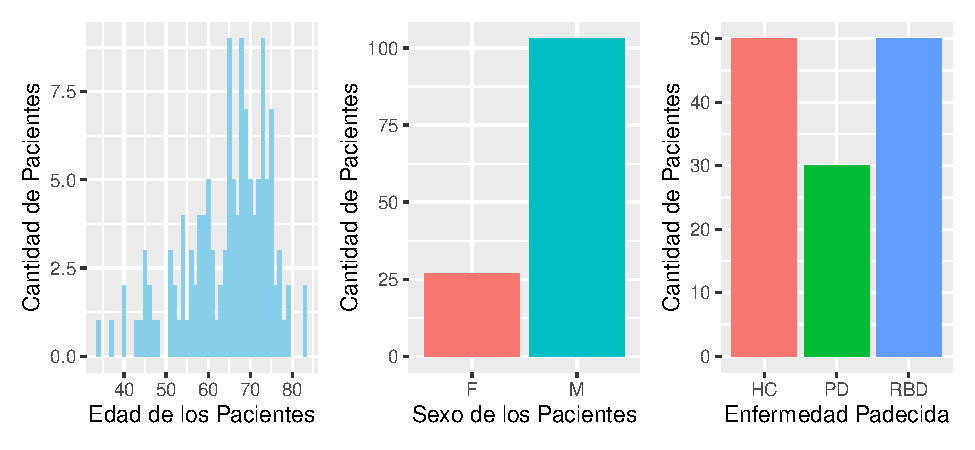
\includegraphics{Ej_AD_2_files/figure-latex/unnamed-chunk-11-1.pdf}

\emph{2.Crea un histograma de las poblaciones estatales.}

\begin{Shaded}
\begin{Highlighting}[]
\FunctionTok{hist}\NormalTok{(murders}\SpecialCharTok{$}\NormalTok{population)}
\end{Highlighting}
\end{Shaded}

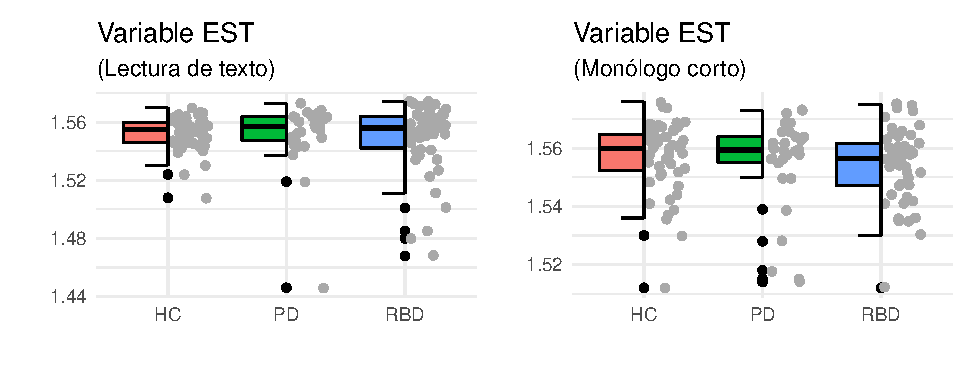
\includegraphics{Ej_AD_2_files/figure-latex/unnamed-chunk-12-1.pdf}

\emph{3.Genere diagramas de caja de las poblaciones estatales por
región.}

\begin{Shaded}
\begin{Highlighting}[]
\FunctionTok{boxplot}\NormalTok{(population}\SpecialCharTok{\textasciitilde{}}\NormalTok{region, }\AttributeTok{data =}\NormalTok{ murders)}
\end{Highlighting}
\end{Shaded}

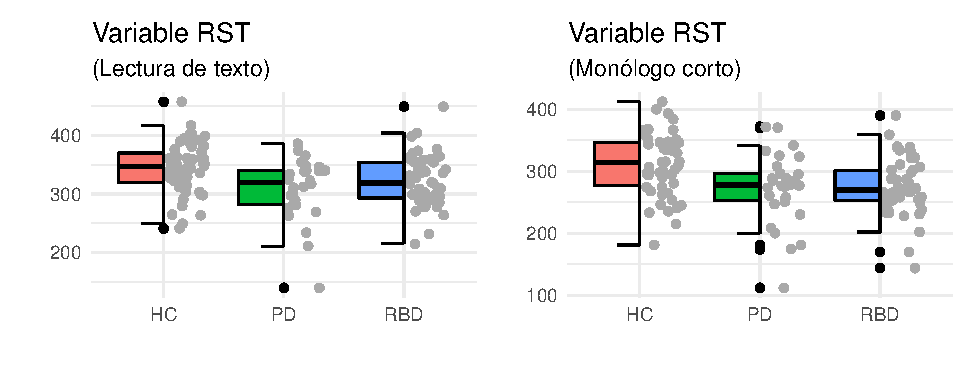
\includegraphics{Ej_AD_2_files/figure-latex/unnamed-chunk-13-1.pdf}

\end{document}
